\documentclass[11pt,a4paper]{article}

\usepackage[T1]{fontenc}
\usepackage[utf8]{inputenc}
\usepackage{lmodern}
\usepackage[margin=2.6cm]{geometry}
\usepackage{amsmath,amssymb}
\usepackage{booktabs}
\usepackage{microtype}
\usepackage{tikz}
\usepackage{caption}
\usepackage[colorlinks=true,linkcolor=blue!50!black,citecolor=blue!50!black,
            urlcolor=blue!50!black]{hyperref}

\newcommand{\dd}{\mathrm{d}}
\newcommand{\ed}{\boldsymbol{e}_d}
\newcommand{\nn}{\boldsymbol{n}}
\newcommand{\grad}{\boldsymbol{\nabla}}
\newcommand{\code}[1]{\texttt{#1}}

\title{Conjugate heat transfer at an immersed interface:\\
       \large the scheme as implemented}
\author{As-built note --- what the solver does today}
\date{}

\begin{document}
\maketitle

\begin{abstract}
\noindent
This note describes the conjugate-heat-transfer scheme \emph{as it exists in
the code}. It is deliberately narrower than the design note
\code{conjugate\_ibm.tex}, which surveys three source methods, derives the
exact cut-face flux including its tangential term, works out a corner model,
and weighs alternatives. None of that survey is repeated here. What is
described here is what runs: one face coefficient, a fluid-fraction-weighted
capacity, a time-step bound, a configuration surface with five hard guards, and
two diagnostics. Where a term exists in the code but is switched off by
default, it is stated as such together with the measurements that decided it
(\S\ref{sec:disabled}); where a piece of the design was never built, it is
listed so that the reader is not misled (\S\ref{sec:notbuilt}).
\end{abstract}

%======================================================================
\section{What is solved}
%======================================================================

The solid stops being a boundary condition and becomes a real unknown. Fluid
and solid carry the same scalar variable, advanced by the same kernel, and
differ only through two ratios that are $1$ in the fluid by definition:
\[
  \kappa \;=\; \frac{k}{k_f},
  \qquad
  C \;=\; \frac{(\rho c)}{(\rho c)_f}.
\]
In the solver's non-dimensional form, with $D_f = 1/(Re\,Pr)$ the fluid
diffusivity, the transported scalar $s$ obeys
\begin{equation}
  C\,\partial_t s
  \;=\;
  -\,\grad\!\cdot\!\left(\boldsymbol{u}\,s\right)
  \;+\;
  \grad\!\cdot\!\left(\kappa D_f \grad s\right)
  \;+\; C\,q ,
  \label{eq:pde}
\end{equation}
with $\boldsymbol{u}\equiv\boldsymbol{0}$ and $\kappa=\kappa_s$, $C=C_s$ inside
the body. At the interface the physical conditions are continuity of
temperature and of normal flux,
\begin{equation}
  s_f = s_s,
  \qquad
  k_f\,\partial_n s_f = k_s\,\partial_n s_s ,
  \label{eq:interface}
\end{equation}
optionally relaxed to a contact resistance $R_c$ (\S\ref{sec:coefficient}).
\textbf{Neither condition is imposed anywhere in the code.} They are
consequences of a single face coefficient, which is the whole scheme.

%======================================================================
\section{Geometry: one stored field}
\label{sec:geometry}
%======================================================================

The scheme reads exactly one geometric field, and it is one the solver already
produced for the turbulence models:
\begin{equation}
  \varphi \;=\; \pm\,\code{dwall},
  \label{eq:phi}
\end{equation}
the distance to the surface, \emph{signed} negative inside the solid. It is
ghost-inclusive and pointwise exact from the geometry --- no halo exchange is
needed for it, because every value is computed from the surface, not from
neighbours.

The sign comes from the cell-centred immersed-boundary marker: a cell centre
lies in the solid exactly when $|\,\code{coef}(\text{VAR\_P})\,| > 10^{20}$,
because \code{set\_ibm\_coeff} writes $\textsc{solid}/Re$ there and grades only
fluid-centred cells. Both producers of \code{dwall} (the file-based path via
the case file's \code{dwall\_blocks}, and the analytic path) already supply
what is needed; the conjugate mode adds \textbf{no new dataset and no
case-file format change}.

\paragraph{The obliquity lemma.}
This is why no normal vector is ever computed. Let the interface be locally a
plane with unit normal $\nn$, and consider a grid arm along $\ed$ joining two
cell centres at distance $h_d$, with $a = \nn\cdot\ed$ the direction cosine.
Because $\varphi$ stores the \emph{perpendicular} distance,
\[
  \varphi_L = a\,\delta_L, \qquad \varphi_R = -\,a\,\delta_R ,
\]
where $\delta_L,\delta_R$ are the distances \emph{along the arm} from each
centre to the interface. The cosine therefore cancels in the ratio:
\begin{equation}
  \boxed{\;
  w \;=\; \frac{\varphi_L}{\varphi_L-\varphi_R}
      \;=\; \frac{\delta_L}{\delta_L+\delta_R}\;}
  \label{eq:w}
\end{equation}
is the true arm fraction \emph{at any orientation}. That is the entire reason
the scheme needs no new data.

\begin{figure}[t]
\centering
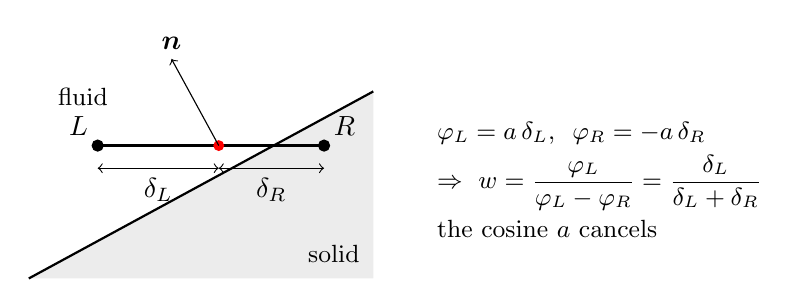
\begin{tikzpicture}[scale=1.25]
  \fill[gray!15] (-0.4,-0.4) -- (3.1,1.5) -- (3.1,-0.4) -- cycle;
  \draw[thick] (-0.4,-0.4) -- (3.1,1.5);
  \node at (2.7,-0.15) {\small solid};
  \node at (0.15,1.45) {\small fluid};
  \draw[very thick,-] (0.3,0.95) -- (2.6,0.95);
  \filldraw (0.3,0.95) circle (1.6pt) node[above left] {$L$};
  \filldraw (2.6,0.95) circle (1.6pt) node[above right] {$R$};
  \draw[dashed] (1.53,0.95) -- (1.53,0.95);
  \filldraw[red] (1.53,0.95) circle (1.4pt);
  \draw[<->] (0.3,0.72) -- (1.53,0.72) node[midway,below] {$\delta_L$};
  \draw[<->] (1.53,0.72) -- (2.6,0.72) node[midway,below] {$\delta_R$};
  \draw[->,thin] (1.53,0.95) -- ++(-0.48,0.88) node[above] {$\nn$};
  \node[align=left] at (5.4,0.6)
    {\small $\varphi_L=a\,\delta_L$, \ $\varphi_R=-a\,\delta_R$\\[1mm]
     \small $\Rightarrow\ w=\dfrac{\varphi_L}{\varphi_L-\varphi_R}
             =\dfrac{\delta_L}{\delta_L+\delta_R}$\\[1mm]
     \small the cosine $a$ cancels};
\end{tikzpicture}
\caption{The obliquity lemma. $\varphi$ stores the perpendicular distance, so
the direction cosine $a$ appears in both signed distances and cancels in their
ratio: $w$ is the arm fraction at any orientation, with no normal computed.}
\end{figure}

%======================================================================
\section{The face coefficient --- the whole scheme}
\label{sec:coefficient}
%======================================================================

At a face whose two cell centres straddle the interface
($\varphi_L\varphi_R<0$), the face diffusivity becomes the
distance-weighted harmonic mean on $w$:
\begin{equation}
  \boxed{\;
    k_{\text{face}}
    \;=\;
    \frac{D_f}{\;\dfrac{w}{\kappa_L}+\dfrac{1-w}{\kappa_R}
          + R_c\,\dfrac{D_f}{h_d}\;}\;}
  \label{eq:kface}
\end{equation}
Every other face keeps today's kernel line verbatim,
$k_{\text{face}} = \kappa_L D_f$. That is the complete interface treatment:
one sign test, one weight, one reciprocal, evaluated inside the flux line the
kernel already had.

What it inherits:
\begin{itemize}
\item \textbf{Exact in one dimension.} It is the series resistance, so it is
      exact for a grid-aligned interface at \emph{any} cut position, and exact
      at any orientation wherever the local gradient is interface-normal.
\item \textbf{Conservative.} It is a face flux --- the neighbour subtracts the
      same number --- so $\sum C\,s\,\Delta V$ is conserved to round-off.
\item \textbf{Correct in both limits.} $\kappa_R\to\infty$ recovers the
      isothermal wall, $\kappa_R\to0$ zero flux.
\item \textbf{Inert when unused.} An uncut face takes the else-branch, which is
      the pre-existing arithmetic operand for operand, so a non-conjugate run
      is bit-identical.
\end{itemize}

\paragraph{Grazing guard.}
$w$ is unreliable for arms nearly \emph{tangent} to the surface, where
$\varphi_L-\varphi_R\to0$. The implementation therefore tests the direction
cosine, which \eqref{eq:w} supplies for free as
$a = |\varphi_L-\varphi_R|/h_d$, and falls back to $w=\tfrac12$ below a
threshold. Such arms carry little of the interface flux, so the fallback costs
nothing measurable.

\paragraph{Contact resistance.}
$R_c$ enters \eqref{eq:kface} as a third resistance in series, which is what it
physically is. It is exact: a gate with $R_c=0.25$ reproduces the analytic
two-material solution to \textbf{$0.0$}.

%======================================================================
\section{The discrete scheme}
%======================================================================

\subsection{Face loop}
The six face diffusivities of a pressure cell are built with \eqref{eq:kface}
and the flux divergence is formed as usual. Nothing else in the diffusion
stencil changes.

\subsection{Convection}
Convection is hard-masked on solid \emph{and} cut faces, and --- this is the
part that is easy to get wrong --- the skew-symmetric term's divergence is
built from the \emph{same} masked velocities. That is what keeps a uniform
scalar exactly preserved, in the solid as well as the fluid.

\subsection{Capacity at cut cells}
The flux divergence is divided by the cell's own volumetric capacity. A cut
cell physically contains both materials, so the capacity is
\textbf{fluid-fraction weighted}:
\begin{equation}
  C_{\text{cell}} \;=\; f + (1-f)\,C_s ,
  \qquad
  \text{rhs} \;=\;
  \frac{-\,\text{conv} + \text{diff} + f\,q_f + (1-f)\,C_s q_s}
       {C_{\text{cell}}} ,
  \label{eq:capacity}
\end{equation}
with $f$ the fluid volume fraction of the cell. The volumetric source is
weighted with the same fraction, as the power density it is.

$f$ is pure geometry, built once at init beside $\varphi$ from the closed
plane-in-box form and stored as \code{vfrac}; it rides the snapshot so a
diagnostic can state the invariant the solver actually conserves. The common
approximation $\mathrm{clip}(\tfrac12+\varphi_c/h)$ is not an approximation of
that form but its degenerate limit --- the one a grid-aligned wall lands in.

\paragraph{Why the weighting is not cosmetic.}
It cannot change any steady state, because it divides a residual that vanishes
there. It is what makes the \emph{transient} second order: with a pointwise
capacity a cut cell carries one material's entire heat capacity, an $O(1)$
error on an $O(h)$ band, i.e.\ first order. Measured on a two-material
eigenmode, against the pre-C3 binary on the same inputs:

\begin{center}
\begin{tabular}{lcc}
\toprule
 & field-error order & decay-rate order \\
\midrule
fluid-fraction weighted (\ref{eq:capacity}) & \textbf{1.99, 2.00} & \textbf{1.99, 2.00} \\
pointwise capacity                          & 1.71, 1.09          & 1.28, 0.54 \\
\bottomrule
\end{tabular}
\end{center}

\subsection{What is deliberately absent}
There is \textbf{no penalization} in the conjugate mode. Its solid cells are
unknowns, not boundary values, so the volume-penalization term that the
\code{dirichlet} mode applies is simply not entered. Likewise $\nu_t$ is
admitted neither in the solid nor at a cut face.

%======================================================================
\section{Time step}
%======================================================================

Two findings, both measured, are built into the explicit bound.

\paragraph{The limit is not the maximum material diffusivity.}
A cut face's $k_{\text{face}}$ can approach $\max(\kappa_L,\kappa_R)$ while
feeding the cell on the \emph{other} side, whose capacity is the other
material's. A fluid cell against a $\kappa_s=1000$ solid therefore sees $1000
\times$ the fluid rate \emph{even when} $\alpha_s=\alpha_f$. The rate is
consequently assembled from the \emph{actual face coefficients} rather than
from $\max(\kappa/C)$ --- which is also some $500\times$ less conservative at
$w=\tfrac12$.

\paragraph{A cut cell attains the Gershgorin bound.}
The uniform interior never excites $\rho \le 2A_{ii}/C_i$; a cut cell does. Its
rate is therefore raised: the implementation uses
\[
  \text{share} \;=\;
  \begin{cases}
    2 & \text{at a cut cell},\\
    6 & \text{otherwise},
  \end{cases}
\]
i.e.\ $\mathrm{d}t \times \tfrac23$ \emph{at cut cells only}. The history is
worth keeping: the first version used $6$ everywhere, C1 halved it to $3$, and
C2 then measured the default sitting at $96\,\%$ of the bound and found an
oblique high-contrast case that went to NaN there. At share $=2$ the margin is
$1.56\times$ and that case runs.

%======================================================================
\section{Configuration surface}
%======================================================================

\begin{center}
\begin{tabular}{ll}
\toprule
key & meaning \\
\midrule
\code{[scalar.N] ibm\_wall = conjugate} & selects the mode (beside
   \code{dirichlet}, \code{adiabatic}) \\
\code{solid\_k}        & $\kappa_s$ \\
\code{solid\_rhocp}    & $C_s$ \\
\code{solid\_init}     & initial solid value \\
\code{solid\_source}   & volumetric source inside the solid \\
\code{contact\_resistance} & $R_c$ in \eqref{eq:kface} \\
\code{tangential\_correction} & the C2 term, \textbf{default off}
   (\S\ref{sec:disabled}) \\
\code{[scalar] indicator\_interval} & the free error indicator \\
\code{[scalar] heat\_interval}      & the interface-heat diagnostic \\
\bottomrule
\end{tabular}
\end{center}

\code{dirichlet} and \code{adiabatic} were left untouched: re-expressing them
through the new arithmetic could not have been bit-exact, and bit-exactness of
the existing modes was worth more than the shared code path.

\paragraph{Five hard configuration errors.}
Each of these silently produces a wrong answer if allowed, so each stops the
run with a message naming the fix:
\code{remove\_solid = true} (the solid must exist);
\code{refine\_body} without \code{keep\_buried} (same);
\code{ibm\_value} on a conjugate scalar (there is no imposed value);
a \code{solid\_*} key on a non-conjugate scalar;
no immersed body at all;
and wall functions. A sixth check is geometric rather than configurational: the
2:1 precondition --- a cut face may not sit on a coarse/fine block face,
because the coefficient is a same-level arm --- is \emph{verified} at init, not
assumed.

%======================================================================
\section{Diagnostics}
%======================================================================

\paragraph{Interface heat (the Nusselt number).}
The conjugate branch sums the scheme's \emph{own} face flux over the cut faces,
with the penalization column explicitly zero --- there is none in this mode,
and \code{coef\_p} is finite in a graded fluid cell, so writing the zero
explicitly forestalls a double count. Gated three ways: against a closed form
($4.6\times10^{-13}$), against an independent Python transcription
($3.6\times10^{-16}$), and against a control-volume budget with the flow on
that falls like $\mathrm{d}t^2$ and does not move with \code{niter}.

\paragraph{The error indicator.}
\code{indicator\_interval} reduces
$e_{\text{face}} = h_d\,s_t/(T_R-T_L)$ over the cut faces (max, rms, count).
This is the closed form of the relative error the scheme makes by dropping the
tangential term, so it is a genuine \emph{a-posteriori} measurement rather than
an assumption, and it is free. It ships enabled.

%======================================================================
\section{Present but disabled: the tangential correction}
\label{sec:disabled}
%======================================================================

The exact cut-face flux carries a second term, $s_t\,(k_{\text{loc}} -
k_{\text{face}})$, which the scheme above drops. It \emph{is} implemented, as
its own flux divergence added after the baseline term --- so it is inert by
construction when off, not by a $+0.0$ argument --- and it is
\textbf{default off}. Three independent measurements decided that:

\begin{enumerate}
\item a crossover ratio $r^\star \approx 0.027$, which the DNS-like
      $|\grad_t T|/|\partial_n T| \sim 10^{-2}$ sits below;
\item an $r=\infty$ boundary-value problem in which the corrected \emph{face
      flux} is exact to $10^{-11}$ while the corrected \emph{field} is
      $2.6\times$ \emph{worse} --- a finite-difference divergence wants the
      face \emph{average}, not the midpoint value;
\item decisively, a cylinder at $\kappa_s=10^3$ where the correction is
      $40$--$65\times$ worse than dropping the term, because
      $|\grad_t T| \propto 2/(1+\kappa_s) \to 0$ in the isothermal limit while
      the discrete estimate of it does not.
\end{enumerate}

The measured fix for (3) --- $k_{\text{area}}$, the face area-weighted mean,
which removes the paradox exactly on a plane --- is recorded but deliberately
not implemented: it cannot rescue the feature, because the binding constraint
is the $s_t$ estimate on curved interfaces. \textbf{Anyone reopening this
starts from $s_t$, not from the multiplier.}

%======================================================================
\section{Not implemented}
\label{sec:notbuilt}
%======================================================================

For the avoidance of doubt, the following appear in the design note and do
\emph{not} exist in the code: the corner/wedge (COCO) model for conducting
sharp corners; the escalation back to the full exact flux as a supported mode;
and any pluggable local-solution interface. The corner model rests on the same
pointwise-flux premise that measurement (2) above falsified, so it should not
be started without first settling the $s_t$ estimate.

%======================================================================
\section{Validation status}
%======================================================================

\paragraph{Manufactured solutions and identities.}
A 1D two-material slab with the cut swept through a full cell and $\kappa_s$
over five decades: $\max|\theta-\theta_{\text{exact}}| \le 9.7\times10^{-15}$
over 28 pairs, and $w$ itself $2.2\times10^{-14}$ against the analytic cut,
rebuilt from the case file without the solver. Capacity-independent steady
state; contact resistance exact; $\sum C\theta\,\Delta V$ drift
$1.2\times10^{-16}$ relative with the flow on. $1$ rank $=4$ ranks and
CPU $=$ GPU at \code{max\_abs 0} on both geometry paths. Every
\code{ibm\_wall} $\ne$ \code{conjugate} run and every \code{[scalar] count = 0}
run bit-exact against the pre-feature binaries.

\paragraph{Turbulence.}
A conjugate channel at $Re_\tau=149$, $Pr=0.71$, matched to Flageul et al.\
(2015) in thermal problem, Reynolds number, grid resolution, solid thickness
and outer-wall boundary condition, compared against \emph{their published raw
data}. Agreement, as a percentage of each quantity's own peak:
\begin{center}
\begin{tabular}{lclc}
\toprule
$U^+$ & $0.5\,\%$ & $\overline{u'v'}$ & $0.6\,\%$ \\
$\theta^+$ & $1.1\,\%$ & $\overline{u'T'}$ & $1.1\,\%$ \\
$\overline{u'^2}$ & $1.0\,\%$ & $\overline{v'^2}$ & $2.2\,\%$ \\
$\overline{w'^2}$ & $4.3\,\%$ & $\overline{T'^2}$ & $2.2\,\%$ \\
\bottomrule
\end{tabular}
\end{center}
The velocity comparison matters independently: it is the first against a
trustworthy reference, so the thermal agreement is not resting on a
compensating error in the flow.

\end{document}
